\documentclass[11pt]{article}
\usepackage{amsmath, amssymb, amsthm}
\usepackage[retainorgcmds]{IEEEtrantools}

\usepackage[pdftex]{graphicx}
\usepackage{tikz}
\usepackage{circuitikz}
\usetikzlibrary{intersections}

\usepackage{fancyhdr}

%Format stuff
\pagestyle{fancy}
\headheight 35pt

%Header info
\chead{\Large \textbf{Interference and Diffraction}}
\lhead{}
\rhead{}

\begin{document}
\section{Two Beam Interference}
	Imagine two identical beams (modeled by traveling waves) pointed at the same point:
	\begin{center}
	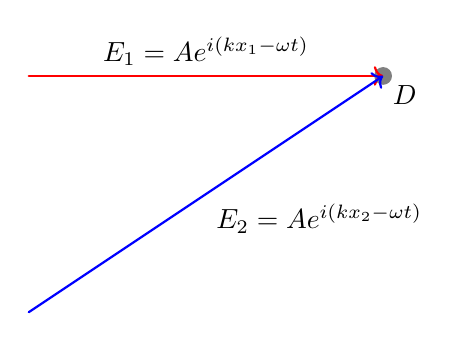
\begin{tikzpicture}
		[scale=1.5,line cap=round,
		%Styles
		axes/.style=,
		important line/.style={very thick},
		information text/.style={rounded corners,fill=red!10,inner sep=1ex},
		dot/.style={circle,inner sep=1pt,fill,label={#1},name=#1}			
		]
		
		%Colors
		\colorlet{anglecolor}{green!50!black}	%angle arcs/lines
		
		%The graphic
		\filldraw[color=gray] (3, 0) node[below right,black] {$D$} circle (2pt);
		\draw[->,thick,red] (0, 0) -- node[above,black] {$E_1 = Ae^{i(kx_1-\omega t)}$} (3, 0);
		\draw[->,thick,blue] (0, -2) -- node[below right,black] {$E_2 = Ae^{i(kx_2 - \omega t)}$} (3, 0);
	\end{tikzpicture}
	\end{center}
	These two beams will exhibit interference at $D$. The combined wave at that point is then
	\begin{IEEEeqnarray}{rCl}
		E_p = E_1 + E_2 & = & 2Ae^{i(k\bar{x} - \omega t)}\cos\left( \frac{k\delta}{2} \right)\\
		\delta & = & x_2 - x_1\\
		\bar{x} & = & \frac{x_1 + x_2}{2}
	\end{IEEEeqnarray}
	The cosine term is called the \textbf{amplitude factor} and the exponential is called the \textbf{wave factor}. 
	
	Usually for analysis, we discard the wave factor because it is oscillating too fast to observe. If we only want the amplitude factor, or the \textbf{intensity} of the resultant wave. The intensity is proportional to the amplitude squared, as follows:
	\begin{equation}
		I \propto E_p E_p^* = 4A^2\cos^2\frac{k\delta}{2}
	\end{equation}
	For a single beam, this result would be $A^2$, but the superimposed wave has an amplitude factor that has to be factored in. Note that for interfering beams of equal intensity, the intensity maximum is 4 times what it would be for one beam.
	

%	\begin{center}
%	\begin{tikzpicture}
%		[scale=3,line cap=round,
%		%Styles
%		axes/.style=,
%		important line/.style={very thick},
%		information text/.style={rounded corners,fill=red!10,inner sep=1ex},
%		dot/.style={circle,inner sep=1pt,fill,label={#1},name=#1}			
%		]
%		
%		%Colors
%		\colorlet{anglecolor}{green!50!black}	%angle arcs/lines
%		
%		%The graphic
%	\end{tikzpicture}
%	\end{center}

%	\begin{figure}[htb]
%		\centering
%		\includegraphics[width=0.8\textwidth]{filename.eps}
%		\caption{Caption.}
%		\label{fig:figure}
%	\end{figure}

%		\def\enotesize{\normalsize}
%		\theendnotes
\end{document}